\chapter{Background e Stato dell'Arte}

In questo capitolo vengono presentati i fondamenti concettuali per il riconoscimento dei malware\
sulla base dei loro comportamenti.
Saranno introdotte le due principali tecniche di analisi, statica e dinamica, mettendone in evidenza\
punti di forza e limitazioni.
In seguito, l'attenzione verrà posta sull'analisi dinamica, approccio adottato in questa tesi,\
illustrandone i principi di machine learning adoperati per la sua realizzazione.

\section{Analisi Statica e Dinamica}

L'analisi statica si concentra sull'esame del codice del programma alla ricerca di specifiche sequenze di istruzioni,
denominate \textit{virus signature} (firma del virus)\mycite{christodorescu_jha_2003}.
L'efficacia dei sistemi basati su questa tecnica dipende dalla dimensione e dall'aggiornamento del database delle firme
e dall'impossibilità, per il software, di modificare nel tempo la propria struttura.
Per aggirare tali sistemi di rilevamento, i creatori di malware hanno sviluppato diverse tecniche di offuscamento,
che consentono di generare firme differenti rispetto a quelle originarie, rendendo più complessa la loro individuazione.
Tra le principali tecniche ritroviamo:

\begin{itemize}
      \item \textbf{Dead Code Insertion} (inserimento di codice morto): aggiunta di istruzioni prive di funzionalità
            ai fini malevoli, il cui unico scopo è alterare la firma rilevata\mycite{christodorescu_jha_2003}.
      \item \textbf{Code Transposition} (trasposizione del codice): riordinamento delle istruzioni,
            in modo che la rappresentazione binaria risulti differente pur mantenendo inalterata la logica di esecuzione\mycite{christodorescu_jha_2003}.
      \item \textbf{Register Reassignment} (riassegnazione dei registri): modifica dei registri utilizzati
            nelle operazioni interne al programma\mycite{christodorescu_jha_2003}.
      \item \textbf{Instruction Substitution} (sostituzione delle istruzioni): rimpiazzo di blocchi di codice
            con altri semanticamente equivalenti\mycite{christodorescu_jha_2003}.
\end{itemize}

Il continuo sviluppo di tecniche di offuscamento e l'aggiornamento dei database di firme ha dato vita a un vero e proprio ciclo vizioso,\
in cui l'evoluzione dei malware procede di pari passo con quella dei sistemi di rilevamento.\
Ne consegue che l'analisi statica tende a concentrare gli sforzi non tanto sull'identificazione diretta del codice malevolo,\
quanto piuttosto sulla gestione delle tecniche di offuscamento, finendo così per allontanarsi dal compito primario di rilevare il malware e,\
soprattutto, di coglierne i reali comportamenti.

L'analisi dinamica supera i limiti dell'approccio statico, poiché osserva i comportamenti\
effettivi del software durante l'esecuzione.\
In questo modo non solo riduce l'impatto delle tecniche di offuscamento sul codice,\
ma consente anche di evidenziare quei casi limite che l'analisi statica difficilmente riesce a cogliere,\
risultando complessivamente più efficace\mycite{Cesare2012-it}.
Per poter eseguire un analisi dinamica, esistono diverse tecniche:

\begin{itemize}
      \item \textbf{Hooking} (Aggancio): intercetta chiamate API per monitorare o modificare il comportamento di un\
            programma. Utilizzato spesso dagli antivirus per controllare processi sospetti.\
            Limite: i malware possono rilevare la presenza di hook tramite checksum o controlli interni\mycite{Cesare2012-it}.\
            Un software per intercettare le chiamate API di Windows è \textit{Detours}\mycite{Detours}.

      \item \textbf{Dynamic Binary Instrumentation} (Strumentazione Dinamica del Binario): analizza e modifica\
            il codice binario mentre il programma è in esecuzione, permettendo di osservare ogni istruzione o comportamento\
            in tempo reale. Più difficile da rilevare rispetto all'hooking\mycite{Cesare2012-it}.\
            Un software che permette tale realizzazione è \textit{Dynamorio}\mycite{DynamoRIO_2025}.\

      \item \textbf{Virtualization} (Virtualizzazione): esegue un sistema operativo guest su hardware reale (host) isolato,\
            sfruttando meccanismi di separazione.\
            Veloce e relativamente sicuro, ma alcuni malware possono rilevare VM tramite differenze hardware/software\mycite{Cesare2012-it}.

      \item \textbf{Application Level Emulation} (Emulazione a Livello di Applicazione): crea un ambiente finto che emula\
            il sistema operativo e l'architettura di istruzioni per singole applicazioni.\
            Utile per analisi real-time e unpacking\footnote{Per \textit{unpacking} si intende il processo di estrazione del codice originario}, ma limitato nella fedeltà: i malware possono rilevare l'emulazione\
            usando istruzioni o API rare\mycite{Cesare2012-it}.

      \item \textbf{Whole System Emulation} (Emulazione dell'Intero Sistema): emula completamente l'hardware di un PC,
            permettendo l'installazione di un intero sistema operativo guest.\
            Molto utile per osservare comportamenti complessi, unpacking e analisi dettagliata, ma più lento rispetto alla virtualizzazione\mycite{Cesare2012-it}.
\end{itemize}

Un esempio concreto di implementazione della tecnica di \textbf{hooking} è presentato nell'articolo di \textit{Wtrace}\mycite{wtrace_net_2023},\
dove l'utilizzo della libreria \textit{Detours} permette di intercettare le chiamate API di un processo in esecuzione.\
Il risultato di tale analisi può essere osservato nella Figura~\ref{fig:api_call_example}, che mostra un output delle API Call registrate\
di un programma in esecuzione:\

\begin{figure}[htbp]
      \centering
      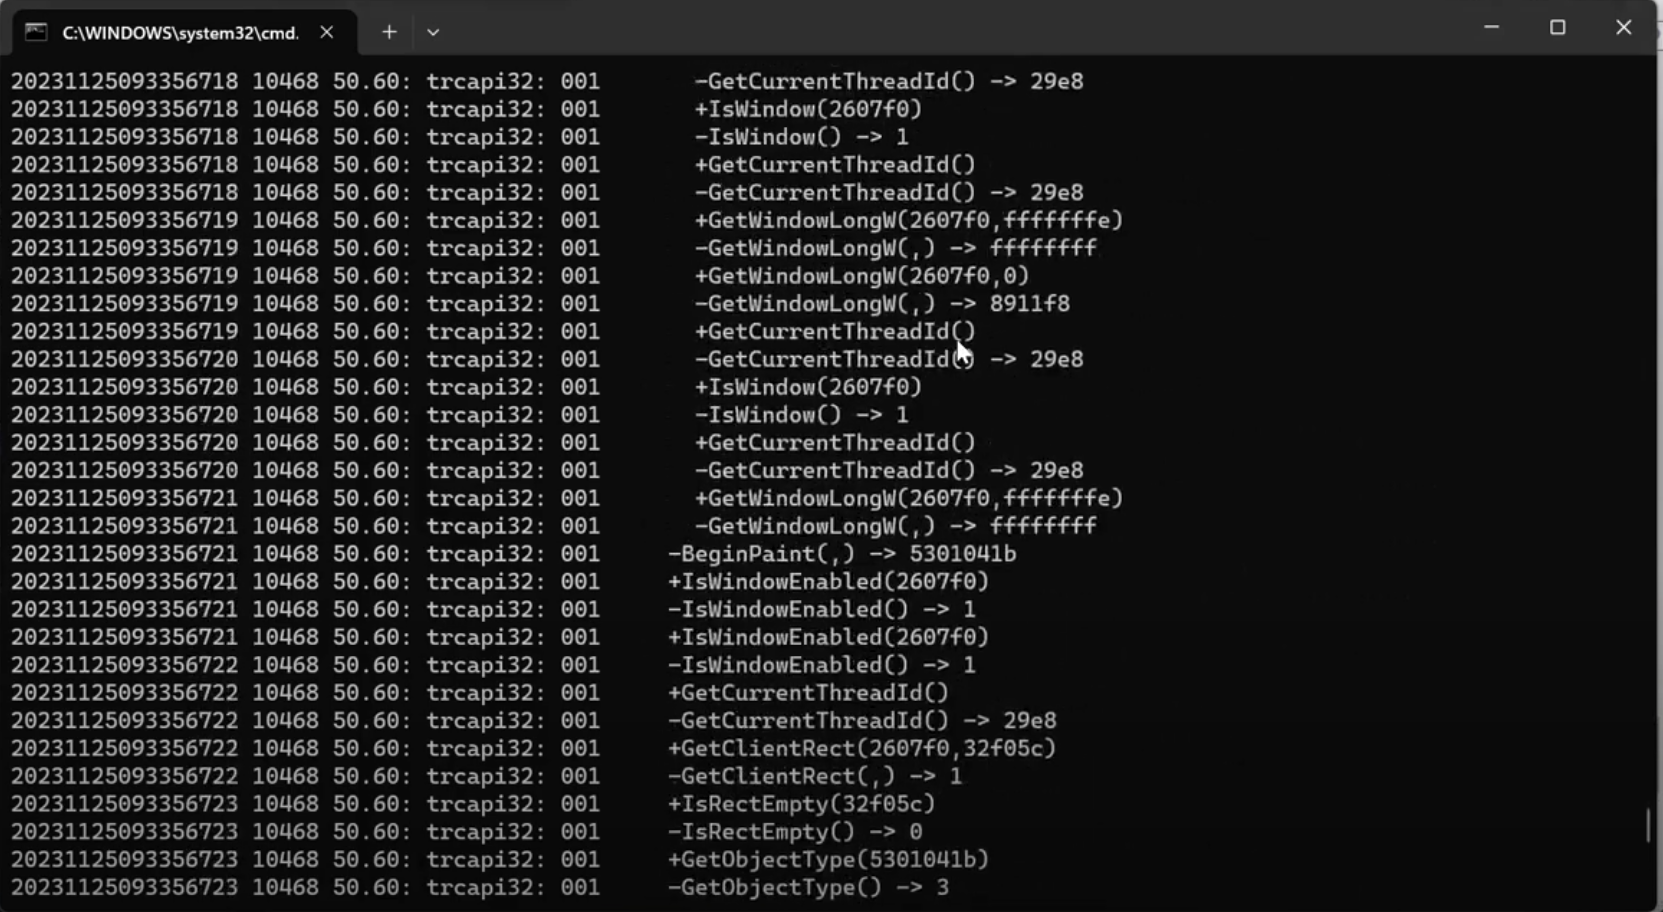
\includegraphics[width=1\textwidth]{./stato-dell-arte/imgs/api_call_example.png}
      \caption{API Call catturate}
      \label{fig:api_call_example}
\end{figure}

Tuttavia, il semplice elenco delle chiamate API non è sufficiente per mostrare la vera natura di un software.\
É necessario definire una logica in grado di estrarre pattern a partire da questi dati in grado di identificare in maniera automatica i comportamenti malevoli.\
In questa tesi\ tali logiche sono implementate tramite \textit{machine learning}.

\section{Machine Learning}

Il \textit{machine learning} (ML) è una branca dell'intelligenza artificiale (IA) che consente a computer e macchine di apprendere dai dati,\
imitando i processi cognitivi umani\mycite{ibm_machine_learning_2025}.\
In termini pratici, il ML consiste nell'\textbf{addestramento} di un software, detto \textbf{modello},\
per svolgere compiti specifici come effettuare \textbf{previsioni} o generare contenuti (testo, immagini, audio o video)\
a partire da dati osservati\mycite{google_ml_intro}.\
\
Un modello di \textit{machine learning} può essere visto come un costrutto matematico che riceve dati in ingresso (\textit{input})\
e produce un risultato (\textit{output}), in modo analogo a una funzione matematica\mycite{google_ml_glossary_modello}.\
L'\textbf{allenamento} di un modello consiste nel processo di identificazione dei parametri ottimali interni,\
così che il modello possa compiere previsioni accurate; ciò avviene fornendogli una serie di esempi\mycite{google_ml_glossary_allenamento}.\
\
Un \textbf{esempio} è un'istanza di input descritta da un insieme di variabili organizzate in un \textbf{vettore delle caratteristiche}
(\textit{feature vector})\mycite{google_ml_glossary_esempio}.\
Ogni variabile è detta \textbf{caratteristica} (\textit{feature}) e rappresenta un'informazione specifica del dominio del problema\mycite{google_ml_glossary_caratteristica}.\
Le caratteristiche possono essere di tipo \textbf{numerico}, quando esprimono valori quantitativi,\
oppure \textbf{categorico}, quando descrivono attributi qualitativi.\
Un insieme di esempi costituisce un \textit{dataset}.

I modelli di \textit{machine learning}, in base al tipo di addestramento e ai dati disponibili,\
possono essere suddivisi in quattro categorie principali:

\begin{itemize}
      \item \textbf{Apprendimento supervisionato}: il modello impara a fare previsioni a partire da dati etichettati,\
            ossia accompagnati dalle risposte corrette, scoprendo le relazioni tra input e output\mycite{google_ml_intro}.
      \item \textbf{Apprendimento non supervisionato}: il modello lavora con dati privi di etichette e ha come obiettivo l'identificazione di strutture o pattern nascosti nei dati\mycite{google_ml_intro}.
      \item \textbf{Apprendimento per rinforzo}: il modello interagisce con un ambiente, ricevendo feedback sotto forma di ricompense o penalità,\
            e sviluppa progressivamente una strategia ottimale per il raggiungimento di un obiettivo\mycite{google_ml_intro}.
      \item \textbf{Apprendimento generativo}: i modelli non si limitano a classificare o predire, ma generano nuovi contenuti (testo, immagini, audio, ecc.)\
            a partire dagli input forniti dall'utente\mycite{google_ml_intro}.
\end{itemize}

In questa tesi ci concentreremo sull'\textbf{apprendimento supervisionato}, affrontando in particolare il compito di \textbf{classificazione}.

\section{Classificazione}

Il compito di \textbf{classificazione} rientra tra quelli affrontabili tramite \textit{apprendimento supervisionato}.\
In questo paradigma, gli esempi utilizzati durante l'addestramento sono accompagnati dall'output corretto, detto\
\textbf{etichetta} (label)\mycite{google_ml_glossary_etichetta}. Nel caso specifico della classificazione, l'etichetta\
corrisponde a una \textbf{classe}, ossia il valore discreto che identifica a quale categoria appartiene l'esempio.\
Allenando quindi un modello su un dataset etichettato, l'obiettivo della classificazione è predire la classe corretta\
di un nuovo esempio non etichettato.

Esistono molteplici compiti di classificazione, distinti uno dall'altro dal numero delle classi da distinguere e da quanto sono\
mutualmente esclusivi\mycite{Belcic_2025}.

\begin{itemize}
      \item \textbf{Classificazione binaria}: le classi tra cui predire sono due e mutualmente esclusive\mycite{Belcic_2025}.
      \item \textbf{Classificazione multi classe}: le classi tra cui predire sono più di due e mutualmente esclusive\mycite{Belcic_2025}.
      \item \textbf{Classificazione a multipla etichetta}: un esempio può appartenere a più classi\mycite{Belcic_2025}.
\end{itemize}

In questo lavoro di tesi verrà affrontata la classificazione multi classe.

\subsection{Algoritmi di Classificazione}

Esistono molteplici algoritmi per la classificazione, in questa tesi verranno affrontanti \textit{XGboost} e \textit{Random forest}.

\subsubsection{Random forest}

Prima di introdurre l'algoritmo di apprendimento \textit{random forest}, è utile esaminare due concetti
fondamentali alla sua comprensione: \textit{bagging} e \textit{decision tree}.

L'algoritmo di apprendimento \textit{bagging} appartiene alla categoria dei metodi di\
\textbf{apprendimento d'insieme}, il cui obiettivo è ridurre la varianza\footnote{La varianza si riferisce\
      alla sensibilità del modello rispetto alle fluttuazioni nei dati di addestramento\mycite{Mucci_2025}.}\
all'interno di un dataset rumoroso\mycite{Bagging_2025}.\
L'apprendimento d'insieme si basa sull'idea che un gruppo di modelli che collaborano possa raggiungere\
prestazioni superiori rispetto a un singolo modello. Questo principio viene spesso associato al concetto\
di ``saggezza delle folle'', secondo cui un insieme di persone fornisce mediamente decisioni migliori di\
quelle di un singolo esperto\mycite{Bagging_2025}.\
Nel \textit{bagging}, i singoli modelli dell'insieme vengono addestrati --- anche in parallelo --- su\
sottoinsiemi del dataset originario, generati tramite campionamento con reinserimento (bootstrap)\mycite{Mucci_2025}.\
Ciò implica che uno stesso esempio possa comparire più volte all'interno di uno o più sottoinsiemi.\
Al termine dell'addestramento, la previsione finale del sistema viene ottenuta aggregando le risposte di\
tutti i modelli. Nel caso della classificazione, la classe predetta corrisponde a quella che ha ricevuto\
il maggior numero di voti.

L'algoritmo \textit{decision tree} è costituito da una serie di domande organizzate gerarchicamente\
a forma di albero. Le domande sono generalmente chiamate \textit{condizioni}, \textit{split} o \textit{test}.\
Ogni nodo interno (non foglia) contiene una condizione, mentre ogni nodo foglia rappresenta una previsione.\
Per effettuare una predizione, si parte dal nodo radice e si percorre l'albero fino a raggiungere un nodo\
foglia, scegliendo il ramo da seguire in base all'esito della condizione presente in ciascun nodo.\
Il percorso che va dalla radice fino alla foglia è chiamato \textit{percorso di inferenza}\mycite{Alberi_decisionali}.

L'algoritmo \textit{Random Forest} è un'estensione dell'algoritmo di \textit{bagging}, in cui i modelli\
interni sono costituiti da \textit{decision tree}. Oltre a essere addestrati su sottoinsiemi casuali degli\
esempi del dataset (\textit{bagging}), ad ogni nodo viene selezionato un sottoinsieme casuale di\
\textit{feature} candidate per effettuare lo \textit{split}. Questo introduce diversità tra gli alberi,\
riducendo la correlazione tra di essi e aumentando la robustezza del modello complessivo\mycite{CheCosEForestaCasuale_2025}.

\subsubsection{XGBoost}

Per una corretta comprensione dell'algoritmo di apprendimento \textit{XGBoost}, è utile\
introdurre preliminarmente l'algoritmo di apprendimento \textit{boosting} e il concetto\
di \textit{ascesa del gradiente}.

Il \textit{boosting} è una tecnica di apprendimento sequenziale in cui più modelli\
vengono addestrati uno dopo l'altro, ciascuno dei quali cerca di correggere gli errori\
commessi dal modello precedente, al fine di ottenere una previsione progressivamente più\
accurata\mycite{CheCoseBoosting_2024}. Il \textit{boosting} appartiene alla categoria degli apprendimenti d'insieme.

La \textit{discesa del gradiente}\mycite{GradientDescent_2025} è un algoritmo di ottimizzazione che permette di trovare i valori ottimali dei
parametri di un modello minimizzando una funzione di costo.
L'idea di base è semplice: si parte da valori iniziali arbitrari per i parametri, si calcola la pendenza (il\
\textit{gradiente}) della funzione di costo in quel punto e si aggiornano i parametri muovendosi nella direzione\
opposta al gradiente, cioè verso la discesa più ripida. Il processo si ripete finché non si raggiunge un minimo\
(locale o globale).\
Un ruolo cruciale è svolto dal \textit{tasso di apprendimento} (\textit{learning rate}), che stabilisce la grandezza\
dei passi: se troppo grande vi è il rischio di superare il minimo, mentre se troppo piccolo l'addestramento\
risulta molto lento. Esistono diverse varianti:\
\begin{itemize}
      \item \textbf{Batch Gradient Descent}: aggiorna i parametri dopo aver visto tutti i dati di addestramento\mycite{GradientDescent_2025}.
      \item \textbf{Stochastic Gradient Descent (SGD)}: aggiorna i parametri dopo ogni esempio, introducendo rumore\
            ma anche la possibilità di sfuggire ai minimi locali\mycite{GradientDescent_2025}.
      \item \textbf{Mini-batch Gradient Descent}: compromesso tra i due, suddivide i dati in piccoli blocchi\mycite{GradientDescent_2025}.
\end{itemize}

L'obiettivo della discesa del gradiente è ridurre progressivamente l'errore, fino a convergere a un set di
parametri che rende il modello il più accurato possibile.

L'algoritmo di apprendimento \textit{XGBoost} si basa sulla tecnica del \textit{boosting}, in cui\
un modello iniziale, l'albero decisionale, viene progressivamente migliorato\
tramite l'uso della \textit{discesa del gradiente}\mycite{KavlakogluRussi_2025}.

\section{Approcci di Machine Learning per Windows PE Malware Detection}

Diversi studi hanno affrontato il problema della rilevazione dei malware in ambiente Windows
basandosi sull'analisi delle chiamate API.

Ad esempio, Zhang et al. (2015) propongono un approccio innovativo per la rilevazione di malware basato sull'analisi dinamica delle sequenze di chiamate API.\
Gli autori applicano algoritmi di allineamento delle sequenze di DNA per identificare somiglianze tra le sequenze di chiamate API\
di programmi legittimi e malware.\
Gli algoritmi di allineamento delle sequenze risolvono il compito di calcolare il costo minimo necessario per trasformare una stringa $a$\
in una stringa $b$, consentendo operazioni di \textit{inserimento} (aggiunta di un carattere) e \textit{rimozione} (eliminazione di un carattere).\
Una delle soluzioni più note a questo problema è l'algoritmo di Smith-Waterman\mycite{smith1981identification}.\
Nello studio, ogni esempio del dataset è rappresentato da un vettore di feature costituito dai costi di allineamento\
calcolati tra una sequenza sconosciuta e tutte le sequenze note del dataset.\
Il modello proposto ha mostrato buone prestazioni nella classificazione dei malware, evidenziando l'efficacia dell'approccio basato sull'allineamento\
delle sequenze di chiamate API\mycite{KiKim_2015}.

Amer e Zelinka (2020) introducono un approccio innovativo che combina tecniche di analisi semantica e modellazione probabilistica delle sequenze di API.\
L'idea si ispira ai metodi utilizzati nell'elaborazione del linguaggio naturale\
(NLP\footnote{\textit{Natural Language Processing} è un ramo dell'intelligenza artificiale che abilita\
      i computer a comprendere e interpretare il linguaggio umano \mycite{Stryker_Holdsworth_2025}}),\
trattando le sequenze di chiamate API come frasi e le singole API come parole.\
Per rendere questa rappresentazione più significativa, gli autori applicano l'algoritmo \textit{Word2Vec}\mycite{Wikipedia_Word2vec},\
che proietta ogni API in uno spazio vettoriale, in cui elementi che compaiono in contesti simili risultano vicini tra loro.\
I vettori così ottenuti vengono successivamente organizzati in gruppi omogenei mediante \textit{k-means clustering}\mycite{Kavlakoglu_Winland_2025},\
un algoritmo non supervisionato che assegna ciascun elemento a un cluster in base alla distanza dal centroide\footnote{Il centroide è il vettore medio di tutti gli elementi che appartengono a un cluster}.\
In questo modo, ogni API originale viene sostituita dall'indice del cluster di appartenenza, riducendo la complessità senza perdere le relazioni semantiche.\
A partire da questa rappresentazione, gli autori costruiscono due matrici di transizione distinte:\
una per le sequenze di software benigno e una per quelle malevole.\
In tali matrici, ciascuna cella rappresenta la probabilità di passare da uno stato $i$ a uno stato $j$.\
Per classificare una nuova sequenza di API, questa viene mappata nella rappresentazione basata sui cluster e analizzata tramite un modello a catene di Markov,\
in cui la transizione dipende unicamente dallo stato corrente.\
Calcolando la probabilità complessiva della sequenza rispetto ai due modelli (goodware e malware),\
la classificazione viene effettuata scegliendo l'ipotesi con la probabilità più elevata.\
I risultati mostrano performance molto promettenti: l'approccio raggiunge un'accuratezza fino al \percc{99} e consente\
di effettuare previsioni precoci già dalle prime chiamate API, dimostrando l'efficacia della combinazione tra rappresentazione semantica e modellazione probabilistica.


Un contributo più recente è quello di Gond e Mohapatra (2025), che affrontano la classificazione dei
malware considerando il fenomeno del \textit{concept drift}, ovvero la capacità dei malware di adattare i propri comportamenti non solo nel tempo,\
ma anche in funzione del contesto di esecuzione, ad esempio il sistema operativo o l'ambiente (virtualizzato o reale) in cui operano.\
Gli autori combinano tecniche di deep learning con meccanismi di adattamento al drift:
le sequenze di API raccolte tramite sandbox vengono trasformate in rappresentazioni linguistiche
tramite n-grammi\footnote{Un \textbf{n-gramma} è una sotto sequenza contigua di n elementi\mycite{Wikipedia_Ngramma}} e filtrate per rilevanza.\
Successivamente, un algoritmo genetico genera varianti delle feature per simulare nuovi schemi comportamentali emergenti.\
La classificazione è affidata a reti neurali artificiali, ricorrenti e convoluzionali CNN (Convolutional Neural Networks)\mycite{IBM_CNN_2025},\
raggiungendo accuratezze fino al \percc{99,5} anche in presenza di mutazioni nei dati.\
L'integrazione del genetic algorithm consente di ridurre la perdita di performance dovuta al concept drift\mycite{Gond_Mohapatra_2025}.

%Nel lavoro ``Dynamic Signature-based Malware Detection Technique Based on API Call Tracing``\mycite{savenko2019dynamic}, gli autori propongono un metodo per\
%l'identificazione di malware basato sulla generazione dinamica di firme.\
%Questo approccio si fonda sul presupposto che i programmi dannosi e quelli benigni possano essere distinti analizzando le loro chiamate API.\
%La firma del comportamento di un programma consiste in due componenti: la frequenza delle chiamate e la natura dell'interazione delle API critiche.\
%Il processo di identificazione si svolge in due fasi principali.\
%La prima fase riguarda la generazione della firma, che non è un singolo elemento, ma una combinazione di due componenti.
%La valutazione quantitativa si basa sulla frequenza delle chiamate API critiche, mentre la valutazione dell'interazione \`e rappresentata \
%da un grafo diretto. Nel grafo, ogni nodo è una classe di API critiche e ogni arco rappresenta il passaggio da una all'altra.\
%Il secondo stadio è la classificazione del programma.
%Inizialmente, la distinzione tra malware e applicazioni benigne \`e
%determinata analizzando la frequenza delle chiamate API critiche
%e usando il test del Chi-quadrato per stabilire il grado di appartenenza a una classe. Se un programma è classificato come malware, viene utilizzato un classificatore Naive Bayes per identificarne la specifica variante o modifica. Le feature per il classificatore sono derivate dal grafo
%comportamentale, e includono il vettore dei gradi dei vertici, il diametro del grafo e il numero di archi.
%Il classificatore determina l'ipotesi pi\`u probabile confrontando i risultati.
%In conclusione, la firma dinamica, composta dalle frequenze delle
%API e dalle caratteristiche del grafo, permette non solo di rilevare un
%programma dannoso, ma anche di classificarlo con precisione
%all'interno della sua famiglia di appartenenza.
\
Nello studio ``Malware Detection based on API Calls Frequency``\mycite{9036219} La metodologia si articola in diverse fasi:\
in primo luogo, le chiamate API sono state estratte dai file e trasformate in un vettore di feature.\
Per ottimizzare il processo di addestramento e rimuovere le funzionalità ridondanti, è stata applicata\
la tecnica di \textit{feature selection} tramite un algoritmo \textit{Random Forest}.\
Questo ha permesso di identificare le $45$ feature più significative.\
Successivamente, questi vettori di feature ottimizzati sono stati utilizzati per addestrare vari algoritmi di machine learning.\
Tra tutti i modelli testati, l'algoritmo\textit{Support Vector Machine} (SVM\mycite{What_is_support_vector_machine_2025}) ha dimostrato le prestazioni migliori,\
raggiungendo un'accuratezza del \percc{93} nel distinguere il malware dai file benigni.

Sono stati provati anche approcci a grafo, come nello studio ``A malware classification method based on directed API call relationships``\mycite{10.1371/journal.pone.0299706}.\
A differenza degli approcci tradizionali che le considerano come una semplice lista, i ricercatori hanno sviluppato un modello che le tratta\
come un \textbf{grafo diretto}. In questo grafo, ogni nodo è una singola API e gli archi direzionali rappresentano l'ordine e la sequenza con cui\
le chiamate vengono eseguite.\
La metodologia si concentra sul modello \textbf{FSGCN} (First-order and Second-order Graph Convolutional Networks),
il quale analizza il grafo su due livelli per estrarre informazioni cruciali.\
A un livello di \textit{primo ordine}, il modello esamina le connessioni dirette tra le API per comprendere la sequenza immediata.
A un livello di \textit{secondo ordine}, analizza le relazioni indirette (percorsi a due passi), per comprendere il contesto più ampio\
del comportamento del programma.\
Questa combinazione di analisi consente di creare un \textbf{vettore di feature} unificato,\
che racchiude sia i dettagli della sequenza che il contesto relazionale.\
Il vettore di feature viene poi convertito in un'immagine, sfruttando l'efficacia delle \textbf{CNN} per la classificazione finale.\
L'efficacia di questo approccio dimostra che l'analisi delle relazioni strutturali e dell'ordine delle chiamate API\
è un metodo più robusto per la classificazione dei malware.

Questi studi evidenziano come l'analisi delle sequenze di API, se combinata con tecniche di
rappresentazione avanzata e modelli adattativi, possa migliorare sensibilmente l'efficacia della
malware detection in ambienti Windows.